\chapter{Methods\label{chap:Methods}}
% notes: Previous research (discussed in Chapter~\ref{chap:Bkgd}) reveals that virtually any XXX can impact speech perception, and various prosodic dimensions vary with dialect.  Also one limitation of using \psola{} for resynthesis is the limitation of 50Hz / 20ms
%TODO: explain why I used syllablewise duration

\section{The \ac{pn/nc} corpus}
Stimuli for the experiments described here were a subset of the \ac{ieee} “Harvard” sentences \citep{HarvardSents} drawn from the \ac{pn/nc} corpus \citep{xxx}.  The sentences in the \ac{pn/nc} corpus were selected based on absence of alliteration or rhyming, avoidance of focus/contrast readings, and lack of marked locutions; The full list of sentences used is given in Appendix~\ref{apx:HarvardSents}.  

Based on within-dialect intelligibility scores from \citet{McCloyEtAl2013}, three talkers were chosen for the present experiments, herein referred to as talkers \ac{a}, \ac{b}, and \ac{c}.  These talkers were selected from among the Pacific Northwest male talkers because, as a group, the Pacific Northwest male talkers exhibited the largest spread in intelligibility in the corpus, and those three talkers formed the endpoints and midpoint of that group, with talker \ac{a} being the most intelligible and talker \ac{c} the least intelligible (cf. Figure~\ref{fig:dotchart}).

\begin{figure}
	\begin{centering}
	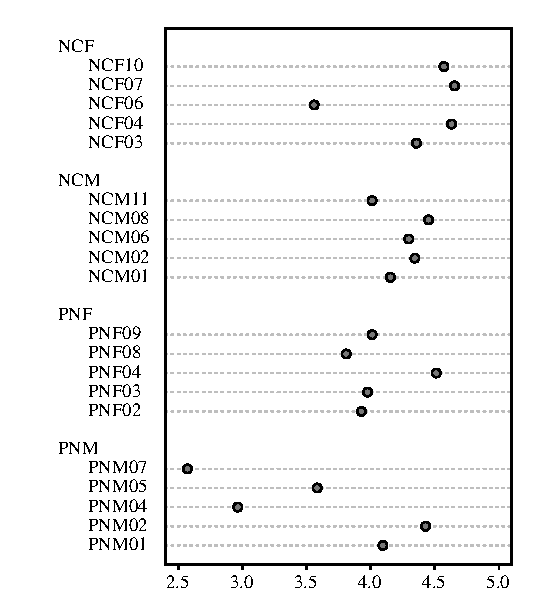
\includegraphics{figures/dotchart.eps}
	\caption[Intelligibility of talkers used to make the stimuli]{By-talker mean keywords correct (across dialect-matched listeners) in speech-shaped noise at +2 dB \ac{snr} (adapted from \citet{McCloyEtAl2013}).\label{fig:dotchart}}
	\end{centering}
\end{figure}

\section{Stimulus design\label{sec:StimDesign}}
Stimuli underwent prosodic replacement, using the \psola{} algorithm as implemented in Praat \citep{praat}.  In all cases, the sentential content of the target file and prosodic donor file were identical (\ie, the recordings were of two different talkers reading the same sentence).  Prosodic replacement requires measurements of duration for both the target file and the prosodic donor file, as well as information about glottal pulse timing of the target file and pitch contour information from the prosodic donor file.

% Why \psola?  Brief comparison of different methods for manipulating duration.  Malah1979 ("linearly combining adjacent intervals of speech to avoid major discontinuities in the waveform"), MoulinesCharpentier1990 (\ac{psola}).  Relate to the studies that used them: PichenyEtAl1989 (Malah method), UchanskiEtAl1996 (segment-by-segment time scaling), LiuZeng2006 (adding silences, "uniform scaling" = \ac{psola}?).  Cf KrauseBraida2002, KrauseBraida2004.

Duration measurements for target and donor files were made at the syllable level.  Syllable boundary marks were based primarily on local minima in the intensity contour of the sentence, with secondary reliance on inflection points in the intensity contour or waveform envelope, or aspects of waveform or spectrogram morphology, when intensity contour minima were absent from the syllable transition region.  The segmentation process was aided by a custom Praat script (see Script~\ref{scr:SyllIntens}).\footnotemark{}

\footnotetext{In cases where intensity contour minima disagreed with phonological syllable affinity, the phonological considerations were given priority.  This arose primarily in cases of fricative-stop onset clusters, where the intensity minimum occured during the stop closure, effectively grouping the fricative into the coda of the preceding syllable.  In such cases, the lack of aspiration on the stop is taken as evidence that it is not in syllable-initial position, and that the syllable boundary should therefore fall before the fricative.}

This method of segmentation was chosen over two competing methods more commonly seen in the literature: marking only periodic/aperiodic transitions, or marking all segmental boundaries.  Both of the more common methods had the drawback of numerous inter-talker differences in the number of durational units in a given sentence, whereas virtually all sentences in the corpus showed inter-talker agreement on number of syllables.  The rare disagreements were cases of extreme reduction, \eg, “It is hard to erase blue or red ink”, in which one talker contracted the initial syllables to “It’s”.  In most such cases, it was still possible to separate the reduced form into two syllable-like units using the same acoustic landmarks mentioned above, and such sentences were therefore retained to avoid introducing a systematic bias by eliminating the most heavily reduced sentences.

Pitch information was measured with Praat using a semi-automated process (see Script~\ref{scr:PulseCor}).  For each recording, pitch tracks generated by Praat’s pitch tracking algorithm were displayed over a narrowband spectrogram, and algorithm parameters were adjusted as necessary to eliminate spurious pulse detections, pitch halving errors, and other irregularities.  The corrected pitch settings were then used to create Praat manipulation objects, which allow manual editing of the detected pulses.  After hand-correction of the pulses, sparse pitch tracks were re-generated with a single pitch value at the midpoint between each pair of pulses in contiguous voicing regions.

Hand-correction of the pulse points was often necessary in recordings involving creaky voicing, either because the frequency dropped below the algorithm’s pitch floor, or because the amount of jitter\slsh{}shimmer present in the creaky voicing exceeded the level at which the algorithm is willing to mark periodicity.  In a small number of cases, extreme jitter and/or shimmer during creaky voicing was suggestive of a very low pitch (\ie, 50 Hz or lower).  In a few such cases, better resynthesis results (judged auditorily) were achieved by marking each cycle — despite cycle-to-cycle irregularities — rather than omitting alternating pulses in order to achieve a smoother, lower-frequency pitch track (see Figure~\ref{fig:JitShim} for illustration).  %It is speculated that the better resynthesis results arise due to more natural waveform period shapes, allowing the simulation of creaky voicing through \term{pitch wobble}, and the partial undoing of creaky voicing through period regularization.
Prior to being mapped onto the target signal, the locations of donor pitch points were shifted via dynamic time warping, with the temporal ratios determined by the relative durations of corresponding syllables in the target and donor files (see Script~\ref{scr:Psola}).

\begin{figure}
	\begin{centering}
	
\includegraphics{figures/xxx.eps}
	\caption[Handling of jitter and shimmer in resynthesis]{Illustration of the method used to accommodate jitter and shimmer in creaky-voiced portions of speech.\label{fig:JitShim}}
	\end{centering}
\end{figure}

Intensity was altered by first multiplying the signal by the difference of the maximum intensity and the inverted intensity contour (see Figure~\ref{fig:IntenManip}), then multiplying the resulting signal by the intensity contour of the replacement prosody and scaling as needed to achieve the desired \ac{rms} amplitude.  To do this, the donor intensity contour first underwent dynamic time warping to match the durational patterns of the target signal (see Script~\ref{scr:Psola}).

\begin{figure}
	\begin{centering}
	
\includegraphics{figures/xxx.eps}
	\caption[Intensity scaling in resynthesis]{Illustration of the method used to scale intensity.\label{fig:IntenManip}}
	\end{centering}
\end{figure}

After resynthesis, all stimuli were assessed auditorily for excessive distortion.  In some cases, problems could be remedied by readjusting the pulse markers and pitch tracks and re-running the resynthesis script; in other cases the problems were irremediable, and the unacceptable donor\slsh{}target\slsh{}sentence combination was excluded from the experimental stimuli.  Most cases of irremediable stimuli arose from one of two sources: intra-syllable segment duration and intensity mismatches (see Figure~\ref{fig:SegDurMismatch}), or complete devoicing of a syllable by the target talker (see Figure~\ref{fig:Devoicing}).

\begin{figure}
	\begin{centering}
	
\includegraphics{figures/xxx.eps}
	\caption[Segment duration mismatch in resynthesis]{Illustration of intra-syllable segment duration and intensity mismatch, which led to unnatural patterns of intensity after resynthesis.\label{fig:SegDurMismatch}}
	\end{centering}
\end{figure}

\begin{figure}
	\begin{centering}
	
\includegraphics{figures/xxx.eps}
	\caption[Syllable devoicing in resynthesis]{Illustration of complete syllable devoicing, which led to unacceptable levels of distortion after resynthesis.\label{fig:Devoicing}}
	\end{centering}
\end{figure}

\section{experiment sessions}
% Rationale for how much training to do:  
% \citep{YonanSommers2000}: Trained talkerID on 4 talkers (2M2F) over 2 days.  Each day: 60 exposure trials, 40 trials training w/ feedback, 60 more exp, 40 more training, 80 test.  All phases were half high-context and half low-context sentences.  End of day 2: single words \& sentences in SNR -5,0,+5, half high- half low-context, half familiar talkers half novel, half male talkers half female.  Familiar/unfamiliar talkers were piloted to make sure they were equally intelligible generally, and to old vs young people.  RESULTS: young listeners near ceiling on talkerID both day1 and day2; old listeners 73\% and 76\%.  Training on sentence material did not aid on the single word task (same as NygaardPisoni1998).  There was a benefit of familiar talker for sentence materials, which was stronger at lower SNRs.  A similar pattern obtained for a second experiment with talker exposure instead of talkerID training.
% \citep{VanEngen2012}: Two 30-minute training sessions (64 sentences) with noise (either SSN, English 2-babble, Mandarin 2-babble) and feedback.  Posttest 1 familiar, 1 unfamiliar talker, half in English babble, half in mandarin.  Trained and tested at their HINT threshold -3dB (based on VanEngen2010) to avoid floor/ceiling.  Results: “(1) listeners were able to take advantage of target talker familiarity; (2) training with babble was more effective than SSN training; and (3) after babble training, listeners improved most in coping with the babble in which they were trained [English or Mandarin]. In general, the results show that processes related both to tuning in to speech targets and tuning out speech maskers can be improved with auditory training”

Except where otherwise noted, stimuli were presented with a stationary gaussian masker noise, frequency shaped to match the long term spectral average of the corpus of stimuli, at 0 dB \ac{snr}.  This \ac{snr} was chosen to avoid ceiling and floor effects, based on a pilot study testing five \ac{snr}s ranging from −1 to +3 dB.  To ensure target audibility, the level of the speech was held constant at 67 dB \ac{spl} (dB \ac{rms} in a 6 cc coupler) and the masker noise was digitally added to the speech to achieve the desired \ac{snr}, yielding a final presentation level of approximately 70 dB \ac{spl}.  The noise extended past the beginning and end of the speech by 50 ms in each direction, and linear onset and offset ramps were applied to this excess noise to prevent clicks during stimulus playback.

The combined speech-and-noise signal was presented in a sound-insulated booth over closed-back supra-aural headphones (Sennheiser HD 25–1 II).  Listeners were instructed to repeat each sentence they heard, to give partial answers when they only heard some words, and to guess when they were unsure.  Trials were scored 0–5 on keywords correct during the task.  An audio recording was made of listener responses, and scoring uncertainties were resolved offline.  

Of the 180 sentences in the corpus, half were set aside for use as training\slsh{}exposure sentences in Experiments~2 and~3; the remaining 90 sentences were designated as test sentences and resythesized versions of those sentences were created.  Experiment~1 presented the 90 test sentences to each listener, with equal numbers of stimuli from each “talker” (\ie, ten from each of the three unmodified talkers \ac{aa}, \ac{bb}, and \ac{cc}, plus ten from each of the six resynthesized “talkers” \ac{ab}, \ac{ac}, \ac{ba}, \ac{bc}, \ac{ca}, and \ac{cb}).  Talker-sentence combinations were random and unique for each listener, subject to the above-mentioned constraints (\ie, each listener heard each talker an equal number of times, and each listener heard each sentence only once).

SUBJECTS
\begin{itm}
	\item{number of listeners}
	\item{hearing test}
	\item{dialect controls}
	\item{demographics: age, gender, ethnicity, geography}
	\item{English native; other languages?}
\end{itm}

\section{data analysis}
Describe data analysis here.
